\documentclass[oneside, 11pt]{article}

\usepackage[T1]{fontenc}
\usepackage[utf8]{inputenc}
\usepackage[dutch]{babel}

\usepackage{fouriernc}
\usepackage[detect-all, load-configurations=binary,
            separate-uncertainty=true, per-mode=symbol,
            retain-explicit-plus, range-phrase={ tot }]{siunitx}

\usepackage{setspace}
\setstretch{1.2}

\setlength{\parskip}{\smallskipamount}
\setlength{\parindent}{0pt}

\usepackage{geometry}
\geometry{marginparwidth=0.5cm, verbose, a4paper, tmargin=3cm, bmargin=3cm, lmargin=2cm, rmargin=2cm}

\usepackage{float}

\usepackage[fleqn]{amsmath}
\numberwithin{equation}{section}
\numberwithin{figure}{section}

\usepackage{graphicx}
\graphicspath{{Figures/}}
\usepackage{subfig}

\usepackage{tikz}
\usetikzlibrary{plotmarks}

\usepackage{fancyhdr}
\pagestyle{fancy}
\fancyhf{}
\rhead{\thepage}
\renewcommand{\footrulewidth}{0pt}
\renewcommand{\headrulewidth}{0pt}

\usepackage{relsize}
\usepackage{xspace}
\usepackage{url}

\newcommand{\figref}[1]{Figuur~\ref{#1}}

\newcommand{\hisparc}{\textsmaller{HiSPARC}\xspace}
\newcommand{\kascade}{\textsmaller{KASCADE}\xspace}
\newcommand{\sapphire}{\textsmaller{SAPPHiRE}\xspace}
\newcommand{\jsparc}{\textsmaller{jSparc}\xspace}
\newcommand{\hdf}{\textsmaller{HDF5}\xspace}
\newcommand{\aires}{\textsmaller{AIRES}\xspace}
\newcommand{\csv}{\textsmaller{CSV}\xspace}
\newcommand{\python}{\textsmaller{PYTHON}\xspace}
\newcommand{\corsika}{\textsmaller{CORSIKA}\xspace}
\newcommand{\labview}{\textsmaller{LabVIEW}\xspace}
\newcommand{\daq}{\textsmaller{DAQ}\xspace}
\newcommand{\adc}{\textsmaller{ADC}\xspace}
\newcommand{\adcs}{\textsmaller{ADC}s\xspace}
\newcommand{\Adcs}{A\textsmaller{DC}s\xspace}
\newcommand{\hi}{\textsc{h i}\xspace}
\newcommand{\hii}{\textsc{h ii}\xspace}
\newcommand{\mip}{\textsmaller{MIP}\xspace}
\newcommand{\hisparcii}{\textsmaller{HiSPARC II}\xspace}
\newcommand{\hisparciii}{\textsmaller{HiSPARC III}\xspace}
\newcommand{\pmt}{\textsmaller{PMT}\xspace}
\newcommand{\pmts}{\textsmaller{PMT}s\xspace}

\DeclareSIUnit{\electronvolt}{\ensuremath{\mathrm{e\!\!\:V}}}

\DeclareSIUnit{\unitsigma}{\ensuremath{\sigma}}
\DeclareSIUnit{\mip}{\textsmaller{MIP}}
\DeclareSIUnit{\adc}{\textsmaller{ADC}}

\DeclareSIUnit{\gauss}{G}
\DeclareSIUnit{\parsec}{pc}
\DeclareSIUnit{\year}{yr}



\title{Weerstation met Arduino}
\author{C.G.N. van Veen}
\docwerkblad{2}{WA}
\version{1.0}

\begin{document}

\maketitle

\section{Weerstation}

\paragraph{Inleiding}
Naast het meten aan kosmische straling met het \hisparc meetstation kunnen  
leerlingen het \hisparc station uitbreiden met een weerstation gemaakt met Arduino.
Dit weerstation heeft als voordeel dat leerlingen dit zelf kunnen bouwen, aanpassen,
programmeren, wind- en water dichtmaken in een box en plaatsen bij het station.
Zo kunnen zij metingen van luchtdruk, buitentemperatuur en temperatuur van de 
detectorplaten meten en correleren met gemeten kosmische straling. Daarnaast 
kan het station uitgebreid worden met andere sensoren zoals UV-index, bliksem, 
regen en windsensoren.

\begin{figure}
    \centering
    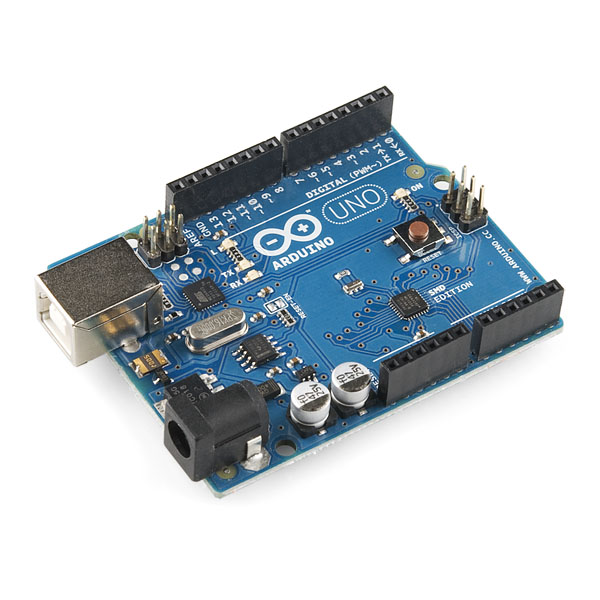
\includegraphics[scale=1.2]{Arduino}
    \caption{Arduino Uno R3, basis voor het weerstation}
   \label{fig:Arduino}
\end{figure}

\paragraph{Benodigdheden}
Het weerstation kan met meer sensoren uitgerust worden dan hier genoemd.
Het basis weerstation (luchtdruk, temperatuur en luchtvochtigheid) waar wij mee
getest hebben heeft de volgende onderdelen nodig: \\
\begin{itemize}
    \item Arduino Uno R3 (of elke andere Arduino)
    \item USB kabel
    \item DTH22 (of DTH11) luchtvochtigheid
    \item BMP085 luchtdruksensor
    \item DS18B20 digitale temperatuursensor (2 of 4x)
    \item APC220 zendmodule
    \item arduino software
\end{itemize}

Andere sensoren zoals een bliksemdetector (AS3935) zijn tot op heden niet getest,
maar geven leerlingen een extra onderzoek mogelijkheid(namelijk de correlatie tussen 
bliksem en kosmische straling.)

\section{Arduino}

\paragraph{werking van Arduino}

Een Arduino is een microcontroller met een ATMEGA-328 chip die bestaat uit 
een printplaatje met een aantal digitale en analoge ingangen, waar bijvoorbeeld  
sensoren op aangesloten kunnen worden. Zie \figref{fig:Arduino}  
Data van de sensoren en via usb of draadloos 
ingelezen worden in de Arduino software. Deze software is vrij te downloaden van
 \url{http://arduino.cc}.
Als u al ervaring heeft met Arduino zal het aansluiten van sensoren redelijk 
eenvoudig zijn. Als er nog geen ervaring is met Arduino zijn er op het internet een 
aantal handleidingen en tutorials beschikbaar evenals Arduino starterskits. 
Het wordt aanbevolen om eerst een aantal basisschakelingen te maken met Arduino.
Voorbeelden van handleidingen zijn te vinden op \url{http://arduino.cc} 
of \url{http://arduino.nu}

Zoals in figuur \figref{fig:Arduino} te zien is zijn er zes analoge ingangen A0-A5 en
zes digitale ingangen (2-7). Voor het basis weerstation zullen we van beide soorten 
twee ingangen gebruiken.
Het voordeel van digitale ingangen is dat zij meerdere waarden kunnen verwerken.
Er kunnen dus meerdere digitale temperatuursensoren (DS18B20) op een digitale 
ingang aangesloten worden. 

De Arduino software heeft een aantal voorbeelden, die de gebruiker snel een aantal zaken leert.
Voor ons is het belangrijk dat we Arduino gebruiken om sensor waarden uit te lezen.
In de Arduino software is dan het voorbeeld: \url{http://http://arduino.cc/en/Tutorial/AnalogReadSerial} 
erg belangrijk. Het voorbeeldprogramma "AnalogReadSerial" bijvoorbeeld 
staat onder file / tools /examples / Basics.
Zie figuur \figref{fig:Arduino_example}  

\begin{figure}
    \centering
    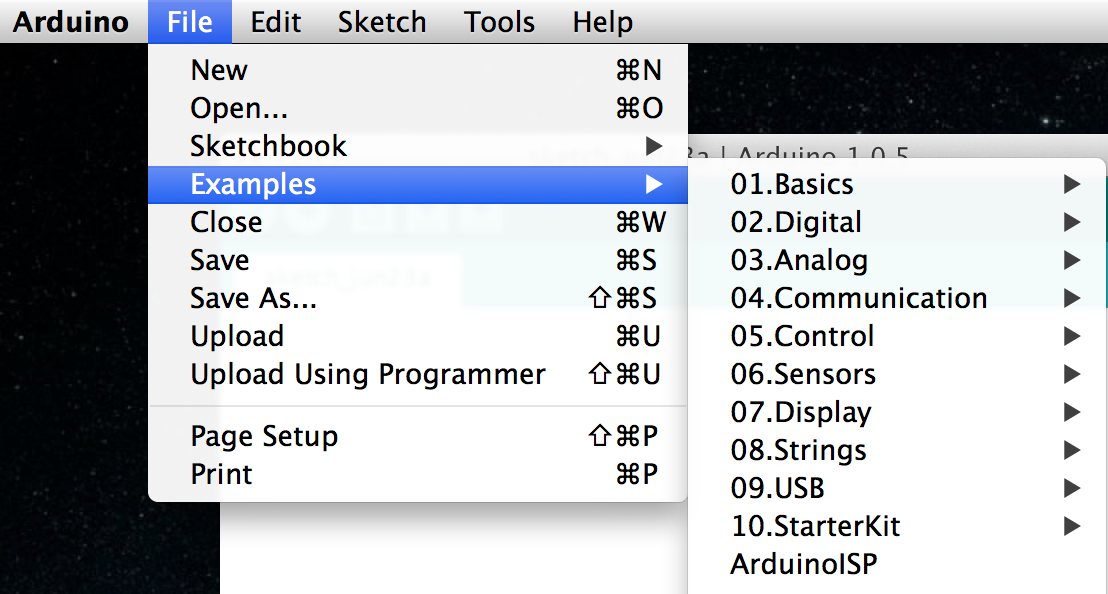
\includegraphics[scale=0.4]{Arduino_example}
    \caption{Arduino Software, voorbeeld programma's}
   \label{fig:Arduino_example}
\end{figure}



\end{document}
